%-------------------------------------------------------------------------
% td-info-S1-instructions.tex
%-------------------------------------------------------------------------

\begin{td}[Unité de pression]\label{td:torr}\index[td]{unité de pression}
\em
Le torr (torr) ou millimètre de mercure (mmHg) est une unité de mesure 
de la pression qui tire son nom du physicien et mathématicien italien Evangelista Torricelli (1608-1647).
Il est défini comme la pression exercée à 0°C par une colonne de 1 millimètre de mercure (mmHg).
Il a plus tard été indexée sur la pression atmosphérique : 1 atmosphère normale correspond à 
760 mmHg et a 101 325 Pa.

Ecrire une instruction qui permette de passer directement des torrs au pascals (Pa).
\end{td}

	\begin{td}[Suite arithmétique (1)]\label{td:suiteArit}\index[td]{suite arithmétique}
\em
	Ecrire une instruction qui calcule la somme $s = \sum_0^n u_k$ des $n$ premiers 
	termes d'une suite arithmétique $u_k = a + r\cdot k$. 
	\end{td}

\begin{td}[Permutation circulaire (1)]\label{td:permutation1}\index[td]{permutation circulaire}
\em
Effectuer une permutation circulaire droite entre les valeurs de 4 entiers $x$, $y$, $z$ et $t$.
\end{td}

\begin{td}[Séquence d'affectations (1)]\label{td:seq1}\index[td]{séquence d'affectations}
\em
Quelles sont les valeurs des variables $a$, $b$, $q$ et $r$ 
après la séquence d'affectations suivante ?
	
	\noindent{\footnotesize\tt
	\mbox{}\ \ a = 19\\
	\mbox{}\ \ b = 6\\
	\mbox{}\ \ q = 0\\
	\mbox{}\ \ r = a\\
	\mbox{}\ \ r = r - b\\
	\mbox{}\ \ q = q + 1\\
	\mbox{}\ \ r = r - b\\
	\mbox{}\ \ q = q + 1\\
	\mbox{}\ \ r = r - b\\
	\mbox{}\ \ q = q + 1
	}
\end{td}

\begin{td}[Opérateurs booléens dérivés (1)]\label{td:booleens1}\index[td]{opérateurs booléens dérivés}
\em
En utilisant les opérateurs booléens de base ({\tt not}, {\tt and} et {\tt or}),
ecrire un algorithme qui affecte successivement à une variable {\tt s} 
le résultat des opérations booléennes suivantes :
ou exclusif ({\em xor}, $a \oplus b$), 
non ou ({\em nor}, $\overline{a+b}$), 
non et ({\em nand}, $\overline{a\cdot b}$), 
implication ($a \Rightarrow b$) et  
équivalence ($a \Leftrightarrow b$).
\end{td}

\index[algo]{circuits logiques}
\begin{td}[Circuit logique (1)]\label{td:circuits}\index[td]{circuits logiques}
\em
Donner les séquences d'affectations permettant de calculer la sortie $s$
du circuit logique suivant en fonction de ses entrées $a$, $b$ et $c$.
$$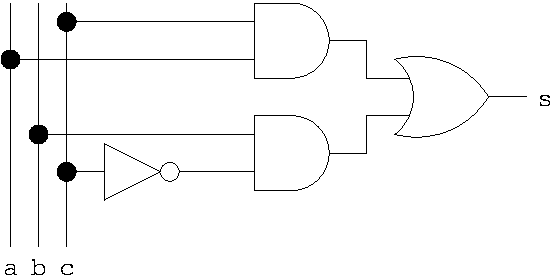
\includegraphics[width=5cm]{mux1.pdf}$$
\end{td}

\begin{td}[Lois de De Morgan]\label{td:prop}\index{{{\sc De Morgan}}}\index[td]{lois de {{\sc De Morgan}}}
\em
Démontrer à l'aide des tables de vérité les lois de De Morgan 
$\forall a, b \in \{0;1\}$ :
\begin{enumerate}
\item {$\overline{(a+b)} = \overline{a} \cdot \overline{b}$} 
\item {$\overline{(a \cdot b)} = \overline{a} + \overline{b}$}
\end{enumerate}
\end{td}


\begin{td}[Maximum de 2 nombres]\label{td:max}\index[algo]{maximum de 2 nombres}\index[td]{maximum de 2 nombres}
\em
Ecrire un algorithme qui détermine le maximum $m$ de 2 nombres $x$ et $y$.
\end{td}

\begin{td}[Fonction « porte »]\label{td:porte}\index[td]{fonction porte}
\em
Proposer une autre alternative simple pour calculer la fonction « porte » de
l'exemple ci-dessous.\\
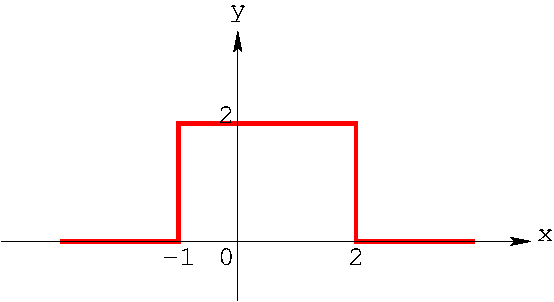
\includegraphics[width=3cm]{porte.pdf}
\end{td}

\begin{td}[Ouverture d'un guichet]\label{td:guichet}\index[td]{ouverture d'un guichet}
\em
A l'aide d'alternatives simples imbriquées, écrire un algorithme qui détermine 
si un guichet est {\tt 'ouvert'} ou 
{\tt 'fermé'} selon les jours de la semaine ({\tt 'lundi'}, {\tt 'mardi'},
\ldots\ ,{\tt 'dimanche'}) et l'heure de la journée (entre 0h et 24h).
Le guichet est ouvert tous les jours de 8h à 13h et de 14h à 17h 
sauf le samedi après-midi et toute la journée du dimanche.
\end{td}

\begin{td}[Catégorie sportive]\label{td:categorie}\index[td]{catégorie sportive}
\em
Ecrire un algorithme qui détermine la catégorie sportive d'un enfant selon
son âge : 
	\begin{itemize}
	\item Poussin de 6 à 7 ans,
	\item Pupille de 8 à 9 ans,
	\item Minime de 10 à 11 ans,
	\item Cadet de 12 ans à 14 ans.
	\end{itemize}
\end{td}

\begin{td}[Dessin d'étoiles (1)]\label{td:etoile}\index[td]{dessin d'étoiles}
\em
Ecrire un algorithme itératif qui affiche les $n$ lignes suivantes (l'exemple
est donné ici pour $n=6$) : \\
\begin{minipage}[t]{2cm}\tt
******\\
*****\\
****\\
***\\
**\\
*
\end{minipage}
\hfill
\begin{minipage}[t]{3cm}
Rappel \python\ : \\
{\tt
\mbox{}\ \ \ \ >>> 5*'r'\\
\mbox{}\ \ \ \ 'rrrrr'\\
\mbox{}\ \ \ \ >>> 2*'to'\\
\mbox{}\ \ \ \ 'toto'
}
\end{minipage}
\end{td}

\begin{td}[Fonction factorielle]\label{td:factorielle}\index[algo]{fonction factorielle}\index[td]{fonction factorielle}
\em
Ecrire un algorithme qui calcule $n! = 1\cdot 2\cdot 3\cdot \ldots \cdot (n-1)\cdot n$.
\end{td}

\begin{td}[Fonction sinus]\label{td:sinus}\index[algo]{développements limités}\index[td]{fonction sinus}
\em
Ecrire un algorithme qui calcule de manière itérative la fonction sinus
en fonction de son d\'eveloppement en série entière.\\
$$\displaystyle\sin(x) \approx \sum_{k=0}^{n} u_k = \sum_{k=0}^{n} (-1)^k\frac{x^{2k+1}}{(2k+1)!} = x - \frac{x^3}{6} + \frac{x^5}{120} + \ldots + (-1)^n\frac{x^{2n+1}}{(2n+1)!}$$
Les calculs seront arr\^et\'es lorsque la valeur absolue du terme $u_k$ sera 
inf\'erieure \`a un certain seuil $s$ ($0 < s < 1$). On n'utilisera ni la fonction 
{\em puissance} ($x^n$) ni la fonction {\em facto\-riel\-le} ($n!$) pour effectuer
le calcul de $\sin(x)$.
\end{td}

\begin{td}[Algorithme d'Euclide]\label{td:euclide}\index[td]{algorithme d'{{\sc Euclide}}}
\em
Dans la tradition grecque, en comprenant un nombre entier comme une longueur, 
un couple d'entiers comme un rectangle, leur pgcd est la taille du plus grand 
carré permettant de carreler ce rectangle. L'algorithme décompose ce rectangle 
en carrés, de plus en plus petits, par divisions euclidiennes successives, 
de la longueur par la largeur, puis de la largeur par le reste, 
jusqu'à un reste nul.\\
Faire la construction géométrique «~à la grecque antique~» qui permet de déterminer 
le pgcd $d$ de $a=21$ et $b=15$ ($d=3$).
\end{td}

\begin{td}[Division entière]\label{td:division}\index[td]{division entière}
\em
Ecrire un algorithme itératif qui calcule le quotient $q$ et le reste $r$ de la 
division entière $a\div b$ ($a = bq+r$).\\
On n'utilisera pas les opérateurs prédéfinis {\tt /} et {\tt \%} mais
on pourra s'inspirer du TD \ref{td:seq1} page \pageref{td:seq1}.
\end{td}


\begin{td}[Affichage inverse]\label{td:caractere}\index[td]{affichage inverse}
\em
Ecrire un algorithme qui affiche les caractères d'une chaîne {\tt s},
un par ligne en partant de la fin de la chaîne.
\end{td}

\begin{td}[Parcours inverse]\label{td:parcours}\index[td]{parcours inverse}
\em
Ecrire un algorithme qui parcourt en sens inverse une séquence {\tt s}
quelconque (du dernier élément au premier élément).
\end{td}
%\begin{fig}[Boucle {\tt for}]\label{fig:for}
%\tt for element in s : blocFor\\
%\centerline{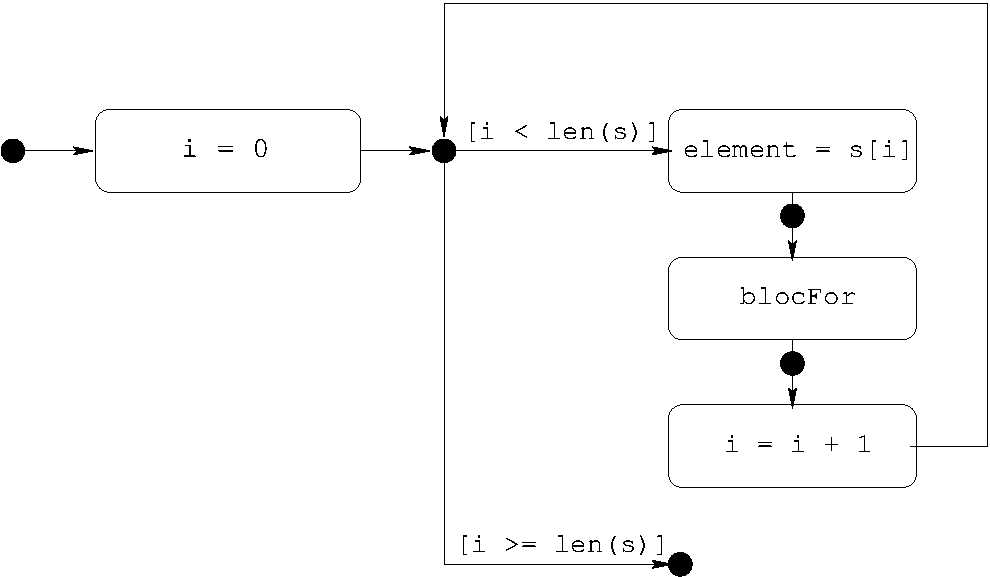
\includegraphics[width=7.5cm]{uml7.pdf}}
%\end{fig}

\begin{td}[Suite arithmétique (2)]\label{td:suiteArit2}\index[algo]{suites numériques}
\em
\begin{enumerate}
\item Ecrire un algorithme qui calcule de manière itérative la somme $s = \sum_0^n u_k$ des $n$ premiers 
	termes d'une suite arithmétique $u_k = a + r\cdot k$. On utilisera une boucle {\tt for}.
\item Comparer l'efficacité de cette approche itérative avec le calcul du TD \ref{td:suiteArit} 
	page \pageref{td:suiteArit}.
\end{enumerate}
\end{td}


\begin{td}[Dessin d'étoiles (2)]\label{td:etoile2}\index[td]{dessin d'étoiles}
\em
Reprendre le TD \ref{td:etoile} page \pageref{td:etoile} en supposant qu'on ne peut 
afficher qu'une étoile à la fois (on s'interdit ici la possibilité d'écrire
{\tt 5*'*'} à la place de {\tt '*****'} par exemple).
\end{td}

\begin{td}[Opérateurs booléens dérivés (2)]\label{td:booleens2}\index[td]{opérateurs booléens dérivés}
\em
A l'aide d'itérations imbriquées, afficher les tables de vérité des 
opérateurs logiques dérivés (voir TD \ref{td:booleens1}) : 
ou exclusif ({\em xor}, $a \oplus b$), 
non ou ({\em nor}, $\overline{a+b}$), 
non et ({\em nand}, $\overline{a\cdot b}$), 
implication ($a \Rightarrow b$) et  
équivalence ($a \Leftrightarrow b$).
\end{td}

\begin{td}[Damier]\label{td:damier}\index[td]{damier}
\em
En utilisant les instructions {\em à la {\sc Logo}} de l'annexe \ref{logo} page \pageref{logo},
dessiner un damier rectangulaire de $n\times m$ cases.
\end{td}

\begin{td}[Trace de la fonction factorielle]\label{td:traceFactorielle}\index[td]{fonction factorielle}
\em
Tracer la fonction factorielle du TD \ref{td:factorielle} page
\pageref{td:factorielle}.
\end{td}

\begin{td}[Figure géométrique]\label{td:quinconce}\index[td]{figure géométrique}
\em
Que dessinent les instructions suivan\-tes ?
\vspace*{1mm}

	{\tt \mbox{}\ \ }\begin{minipage}{5cm}\tt
	x0 = 0\\
	y0 = 0\\
	r = 10\\
	n = 5\\
	m = 10\\
	for i in range(n) :\\
	\mbox{}\ \ \ \ up()\\
	\mbox{}\ \ \ \ y = y0 - 2*r*i\\
	\mbox{}\ \ \ \ x = x0 + r*(i\%2)\\
	\mbox{}\ \ \ \ goto(x,y)\\
	\mbox{}\ \ \ \ for j in range(m) :\\
	\mbox{}\ \ \ \ \ \ \ \ down()\\
	\mbox{}\ \ \ \ \ \ \ \ circle(r)\\
	\mbox{}\ \ \ \ \ \ \ \ up()\\
	\mbox{}\ \ \ \ \ \ \ \ x = x + 2*r\\
	\mbox{}\ \ \ \ \ \ \ \ goto(x,y)
	\end{minipage}
\end{td}

\begin{td}[Suite arithmétique (3)]\label{td:suiteArit3}
Reprendre le TD \ref{td:suiteArit2} page \pageref{td:suiteArit2} en explicitant l'invariant, la condition d'arrêt,
la progression et l'initialisation de la boucle retenue.
\end{td}

\begin{td}[QCM (2)]\label{td:qcmInstruc}\index{evaluation@évaluation!contrôle d'attention}\index[td]{contrôle d'attention}(un seul item correct par question)
\em
\begin{enumerate}
\item En {\sc Python}, l'instruction « ne rien faire » se dit
	\begin{enumerate}
	\item {\tt break}
	\item {\tt return}
	\item {\tt pass}
	\item {\tt continue}
	\end{enumerate}
\item Une variable informatique est un objet 
	\begin{enumerate}
	\item équivalent à une variable mathématique
	\item qui associe un nom à une valeur
	\item qui varie nécessairement
	\item qui modifie la mémoire
	\end{enumerate}
\item L'affectation consiste à
	\begin{enumerate}
	\item comparer la valeur d'une variable à une autre valeur
	\item associer une valeur à une variable
	\item incrémenter une variable
	\item déplacer une variable en mémoire
	\end{enumerate}
\item Après la séquence \fbox{\footnotesize\tt\begin{tabular}{l}a = 13\\b = 4\\b = a\\a = b\end{tabular}} les variables {\tt a} et {\tt b} sont telles que
	\begin{enumerate}
	\item {\tt a = 13} et {\tt b = 13}
	\item {\tt a = 4} et {\tt b = 4}
	\item {\tt a = 4} et {\tt b = 13}
	\item {\tt a = 13} et {\tt b = 4}
	\end{enumerate}
\item Le résultat d'une comparaison est une valeur
	\begin{enumerate}
	\item réelle
	\item qui dépend du type des arguments 
	\item booléenne
	\item entière
	\end{enumerate}
\item Un opérateur booléen s'applique à des valeurs
	\begin{enumerate}
	\item booléennes
	\item entières
	\item réelles
	\item alphanumériques
	\end{enumerate}
\item La fonction principale d'une instruction de test est
	\begin{enumerate}
	\item de passer d'instruction en instruction
	\item de répéter une instruction sous condition
	\item d'exécuter une instruction sous condition
	\item d'interrompre l'exécution d'une instruction
	\end{enumerate}
\item Après la séquence \fbox{\footnotesize\tt\begin{tabular}{l}x = -3\\if   x < -4 : y = 0\\elif x < -3 : y = 4 - x\\elif x < -1 : y = x*x + 6*x + 8\\elif x < 3 : y = 2 - x\\else : y = -2\end{tabular}} la variable {\tt y} est telle que
	\begin{enumerate}
	\item {\tt y = -1}
	\item {\tt y = 0}
	\item {\tt y = 7}
	\item {\tt y = -2}
	\end{enumerate}
\item L'itération conditionnelle est une instruction de contrôle du flux d'instructions 
	\begin{enumerate}
	\item qui permet d'exécuter une instruction sous condition préalable.
	\item qui est vérifiée tout au long de son exécution. 
	\item qui permet sous condition préalable de répéter zéro ou plusieurs fois la même instruction.
	\item qui permet de choisir entre plusieurs instructions.
	\end{enumerate}
\item On ne sort jamais d'une boucle si la condition d'arrêt 
	\begin{enumerate}
	\item ne varie pas en cours d'exécution.
	\item ne contient pas d'opérateurs booléens.
	\item est toujours fausse.
	\item n'est jamais fausse.
	\end{enumerate}
\item Que vaut {\tt f} à la fin des instructions suivantes si $n = 5$ ?

	\begin{py}{4cm}
	\begin{verbatim}
	f = 0
	i = 1
	while i < n+1:
	    f = f + i
	    i = i + 1
	\end{verbatim}
	\end{py}

	\begin{enumerate}
	\item 6
	\item 10
	\item 15
	\item 21
	\end{enumerate}
\item Une séquence est une suite ordonnée 
	\begin{enumerate}
	\item d'éléments que l'on peut référencer par leur rang.
	\item d'instructions formant un ensemble logique.
	\item d'instructions conditionnelles.
	\item de nombres
	\end{enumerate}
\item Dans la chaîne {\tt s = 'gérard'}, {\tt s[2]} vaut
	\begin{enumerate}
	\item {\tt 'é'}
	\item {\tt 'r'}
	\item {\tt 'gé'}
	\item {\tt 'gér'}
	\end{enumerate}
\item Que vaut {\tt f} à la fin des instructions suivantes si $n = 5$ ?

	\begin{py}{4cm}
	\begin{verbatim}
	f = 1
	for i in range(2,n+1) :
	    f = f * i
	\end{verbatim}
	\end{py}

	\begin{enumerate}
	\item 120
	\item 720
	\item 6
	\item 24
	\end{enumerate}
\item Que vaut {\tt f} à la fin des instructions suivantes si $n = 5$ ?

	\begin{py}{4cm}
	\begin{verbatim}
	f, f1, f2 = 2,1,1
	for i in range(3,n+1) :
	    f2 = f1
	    f1 = f
	    f = f1 + f2
	\end{verbatim}
	\end{py}

	\begin{enumerate}
	\item 3
	\item 5
	\item 8
	\item 13
	\end{enumerate}
\end{enumerate}
\end{td}


\begin{td}[Unité de longueur]\label{td:al}\em \index[td]{unité de longueur}
L'année-lumière (al) est une unité de distance utilisée en astronomie. 
Une année-lumière est la distance parcourue par un photon (ou plus simplement la lumière) 
dans le vide, en dehors de tout champ gravitationnel ou magnétique, en une année julienne 
(365,25 jours). 

Ecrire une instruction qui permette de passer directement des années-lumière aux m/s sachant que
la vitesse de la lumière dans le vide est de 299 792 458 m/s.
\end{td}

\begin{td}[Permutation circulaire (2)]\label{td:permutation2}\em \index[algo]{permutation circulaire}\index[td]{permutation circulaire}
 Effectuer une permutation circulaire gauche entre les valeurs de 3 entiers $x$, $y$ et $z$.
\end{td}

\begin{td}[Séquence d'affectations (2)]\label{td:seq2}\em \index[td]{séquence d'affectations}
	Quelles sont les valeurs des variables $n$ et $s$
	après la séquence d'affectations suivante ?
	
	\noindent{\footnotesize\tt
	\mbox{}\ \ n = 1\\
	\mbox{}\ \ s = n\\
	\mbox{}\ \ n = n + 1\\
	\mbox{}\ \ s = s + n\\
	\mbox{}\ \ n = n + 1\\
	\mbox{}\ \ s = s + n\\
	\mbox{}\ \ n = n + 1\\
	\mbox{}\ \ s = s + n\\
	\mbox{}\ \ n = n + 1\\
	\mbox{}\ \ s = s + n
	}
\end{td}

\begin{td}[Circuits logiques (2)]\label{td:circuits2}\em \index[algo]{circuits logiques}\index[td]{circuits logiques}
On considère les conventions graphiques traditionnelles pour les opérateurs logiques :
$$\begin{tabular}{ccccccc}
$\overline{a}$ & $a \cdot b$ & $a + b$ & $a \oplus b$ & $a \cdot b \cdot c$ & $a + b + c$ & $\overline{a \cdot b \cdot c}$ \\
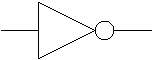
\includegraphics[height=1cm]{non.pdf} & 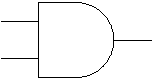
\includegraphics[height=1cm]{et.pdf} & 
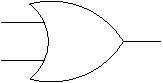
\includegraphics[height=1cm]{ou.pdf}  & 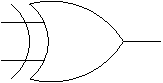
\includegraphics[height=1cm]{xor.pdf} & 
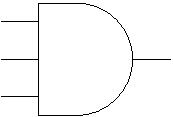
\includegraphics[height=1cm]{et3.pdf} & 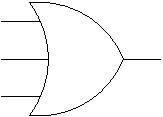
\includegraphics[height=1cm]{ou3.pdf} & 
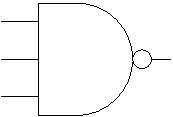
\includegraphics[height=1cm]{nonet3.pdf}
\end{tabular}$$
Donner les séquences d'affectations permettant de calculer la (ou les) sortie(s)
des circuits logiques suivants en fonction de leurs entrées.

\begin{minipage}[t]{7cm}
\begin{enumerate}
\item $a$ et $b$ sont les entrées, $s$ la sortie.
	$$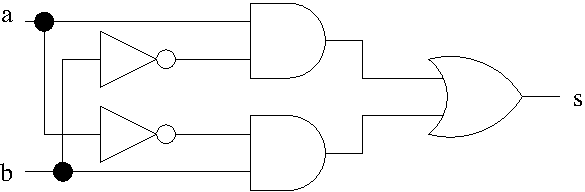
\includegraphics[width=6cm]{ex1.pdf}$$
%\end{enumerate}
%\end{minipage}
%\hfill
%\begin{minipage}[t]{7cm}
%\begin{enumerate}\setcounter{enumi}{1}
\item $a$ et $b$ sont les entrées, $s$ la sortie.
	$$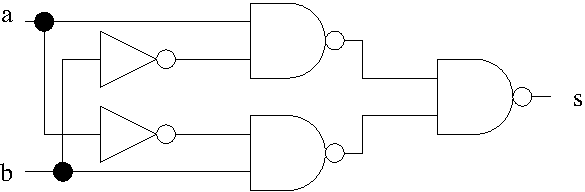
\includegraphics[width=6cm]{ex2.pdf}$$
\end{enumerate}
\end{minipage}
\hfill
\begin{minipage}[t]{7cm}
\begin{enumerate}\setcounter{enumi}{2}
\item $a$ et $b$ sont les entrées, $s$ et $t$ les sorties.	
	$$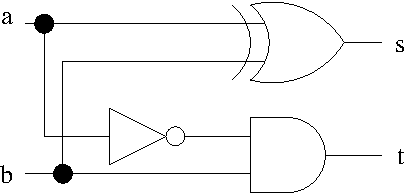
\includegraphics[width=4.5cm]{demiSous.pdf}$$
\item $a$, $b$ et $c$ sont les entrées, $s$ et $t$ les sorties.
	$$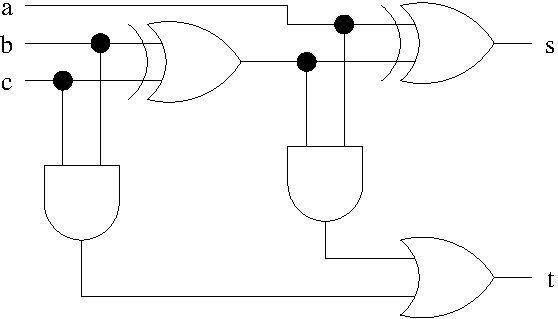
\includegraphics[width=5cm]{add3.pdf}$$
\end{enumerate}
\end{minipage}

\hfill
\begin{minipage}[t]{7cm}
\begin{enumerate}\setcounter{enumi}{4}
\item $a$, $b$ et $c$ sont les entrées et $s$ la sortie.
	$$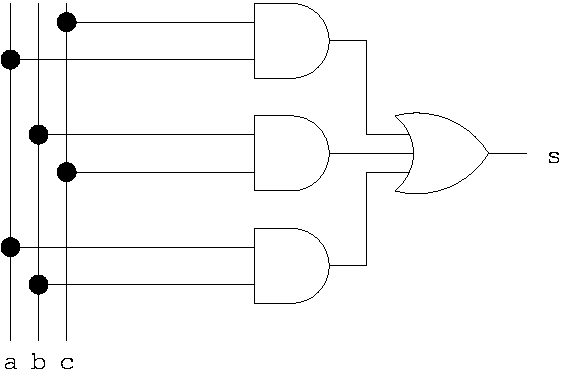
\includegraphics[width=5cm]{majorite.pdf}$$
\item $a$, $b$ et $c$ sont les entrées, $s$ et $t$ les sorties.
	$$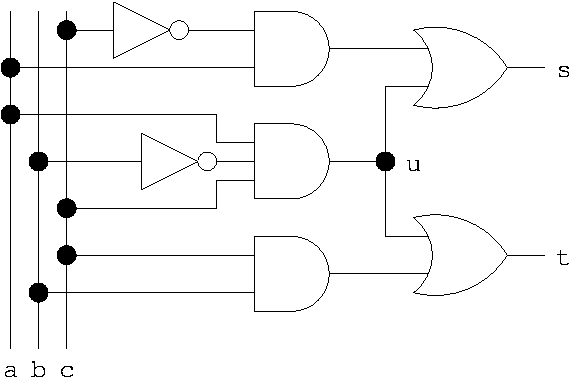
\includegraphics[width=5cm]{circuit.pdf}$$
\end{enumerate}
\end{minipage}
\hfill
\begin{minipage}[t]{7cm}
\begin{enumerate}\setcounter{enumi}{6}
\item $a$, $b$ et $c$ sont les entrées, $s$ la sortie.
	$$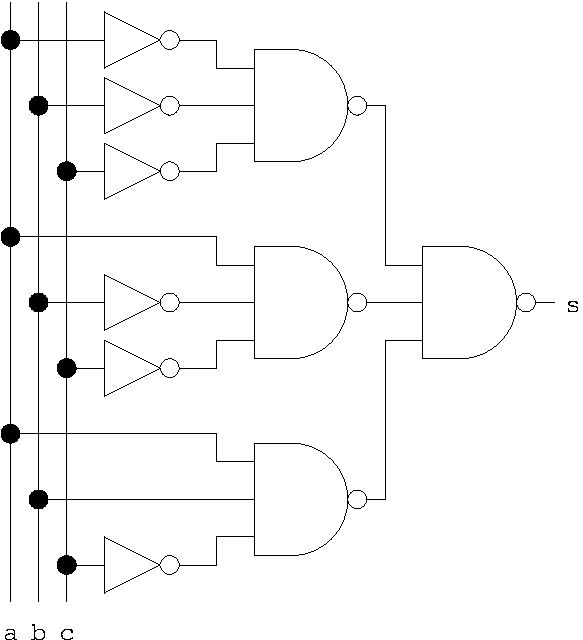
\includegraphics[width=5cm]{f3.pdf}$$
\end{enumerate}
\end{minipage}
\vspace*{3mm}

\begin{minipage}[t]{7cm}
\begin{enumerate}\setcounter{enumi}{7}
\item $a$, $b$ et $c$ sont les entrées, $s_0$,$s_1$\ldots $s_7$ les sorties.
	$$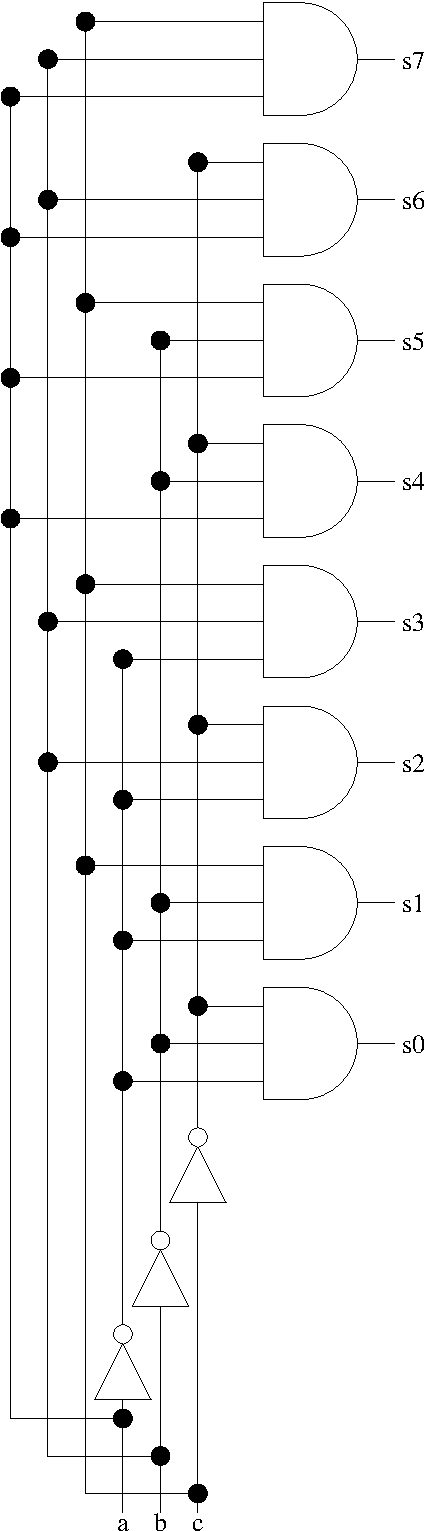
\includegraphics[width=4cm,angle=-90]{decodeur.pdf}$$
\end{enumerate}
\end{minipage}
\end{td}

\begin{td}[Alternative simple et test simple]\label{td:reciproque}\em \index[td]{alternative simple et test simple}
Montrer à l'aide d'un contre-exemple que l'alternative simple :\\
{\tt
\mbox{}\ \ if condition : blocIf\\
\mbox{}\ \ else : blocElse
}\\
n'est pas équivalente à la séquence de tests simples suivante :\\
{\tt
\mbox{}\ \ if condition : blocIf\\
\mbox{}\ \ if not condition : blocElse
}
\end{td}

\begin{td}[Racines du trinome]\label{td:trinome}\em \index[algo]{racines du trinome}\index[td]{racines du trinome}
Ecrire un algorithme qui calcule les racines $x_1$ et $x_2$ du trinome $ax^2 + bx + c$.
\end{td}

\begin{td}[Séquences de tests]\label{td:seq3}\em \index[td]{séquences de tests}
\begin{enumerate}
\item Quelle est la valeur de la variable $x$ après la suite
	d'instructions suivante ?

	{\footnotesize\tt
	x = -3\\
	if x < 0 : x = -x
	}
\item Quelle est la valeur de la variable $y$ après la suite
	d'instructions suivante ?

	{\footnotesize\tt
	x0 = 3\\
	x = 5\\
	if x < x0 : y = -1\\
	else : y = 1
	}
\item Quelle est la valeur de la variable $y$ après la suite
	d'instructions suivante ?

	{\footnotesize\tt
	p = 1\\
	d = 0\\
	r = 0\\
	h = 1\\
	z = 0\\
	f = p and (d or r)\\
	g = not r \\
	m = not p and not z\\
	g = g and (d or h or m)\\
	if f or g : y = 1\\
	else : y = 0
	}
\item Quelle est la valeur de la variable $ok$ après la suite
	d'instructions suivante ?

	{\footnotesize\tt
	x = 2\\
	y = 3\\
	d = 5\\
	h = 4\\
	if x > 0 and x < d :\\
  	\mbox{}\ \ if y > 0 and y < h : ok = 1\\
	\mbox{}\ \ else : ok = 0\\
	else : ok = 0
	}
\item Quelle est la valeur de la variable $y$ après la suite
	d'instructions suivante ?

	{\footnotesize\tt
	x = 3\\
	y = -2\\
	if x < y : y = y - x\\
	elif x == y : y = 0\\
	else : y = x - y
	}
\end{enumerate}
\end{td}
 
\begin{td}[Racine carrée entière]\label{td:racine}\em \index[algo]{racine carrée entière}\index[td]{racine carrée entière}
Ecrire un algorithme qui calcule la racine carrée entière $r$ 
d'un nombre entier positif $n$ telle que $r^2 \leq n < (r+1)^2$.
\end{td}

\begin{td}[Exécutions d'instructions itératives]\label{td:iterations}\em \index[td]{exécutions d'instructions itératives}
\begin{minipage}[t]{7.5cm}
\begin{enumerate}
\item Que fait cette suite d'instructions ?

	{\footnotesize\tt
	x = 0\\
	while x != 33 :\\
	\mbox{}\ \ x = input('entrer un nombre : ')
	}
\end{enumerate}
\end{minipage}
\hfill
\begin{minipage}[t]{7cm}
\begin{enumerate}\setcounter{enumi}{1}
\item Que fait cette suite d'instructions ?

	{\footnotesize\tt
	x = 0\\
	while x <= 0 or x > 5 :\\
	\mbox{}\ \ x = input('entrer un nombre : ')
	}
\end{enumerate}
\end{minipage}

\begin{minipage}[t]{7cm}
\begin{enumerate}\setcounter{enumi}{2}
\item Que fait cette suite d'instructions ?

	{\footnotesize\tt
	s = 0\\
	for i in range(5) :\\
	\mbox{}\ \ x = input('entrer un nombre : ')\\
	\mbox{}\ \ s = s + x
	}
\item Qu'affichent les itérations suivantes ?

	{\footnotesize\tt
	for i in range(0,10) :\\
	\mbox{}\ \ for j in range(0,i) :\\
	\mbox{}\ \ \ \ print('*',end=' ')\\
	\mbox{}\ \ print()
	}
\item Qu'affichent les itérations suivantes ?

	{\footnotesize\tt
	for i in range(0,10) :\\
	\mbox{}\ \ j = 10 - i\\
	\mbox{}\ \ while j > 0 :\\
	\mbox{}\ \ \ \ print('*',end=' ')\\
	\mbox{}\ \ \ \ j = j - 1\\
	\mbox{}\ \ print()
	}
\item Qu'affichent les itérations suivantes ?

	{\footnotesize\tt
	for i in range(1,10):\\
	\mbox{}\ \ for j in range(0,11) :\\
	\mbox{}\ \ \ \ print(i,'x',j,' = ',i*j)\\
	\mbox{}\ \ print()
	}
\item Qu'affichent les itérations suivantes ?\index[algo]{coefficients du binôme}

	{\footnotesize\tt
	for n in range(10) :\\
  	\mbox{}\ \ for p in range(n+1) :\\
    	\mbox{}\ \ \ \ num = 1\\
    	\mbox{}\ \ \ \ den = 1\\
    	\mbox{}\ \ \ \ for i in range(1,p+1) :\\
      	\mbox{}\ \ \ \ \ \ num = num*(n-i+1)\\
      	\mbox{}\ \ \ \ \ \ den = den*i\\
    	\mbox{}\ \ \ \ c = num/den\\
    	\mbox{}\ \ \ \ print(c,end=' ')\\
  	\mbox{}\ \ print()
	}
\end{enumerate}
\end{minipage}
\hfill
\begin{minipage}[t]{7cm}
\begin{enumerate}\setcounter{enumi}{7}
\item Qu'affichent les itérations suivantes ?\index[algo]{nombres de {{\sc Fibonacci}}}

	{\footnotesize\tt
	for n in range(0,15) :\\
  	\mbox{}\ \ f = 1\\
  	\mbox{}\ \ f1 = 1\\
  	\mbox{}\ \ f2 = 1\\
  	\mbox{}\ \ for i in range(2,n+1) :\\
    	\mbox{}\ \ \ \ f = f1 + f2\\
    	\mbox{}\ \ \ \ f2 = f1\\
    	\mbox{}\ \ \ \ f1 = f\\
  	\mbox{}\ \ print(f,end=' ')
	}
\item Quelle est la valeur de la variable $s$
	à la fin des instructions suivantes ?\index[algo]{codage en base $b$}

	{\footnotesize\tt
	b = 2\\
	k = 8\\
	n = 23\\
	s = 0\\
	i = k - 1\\
	q = n\\
	while q != 0 and i >= 0 :\\
  	\mbox{}\ \ s = s + (q\%b)*b**(k-1-i)\\
  	\mbox{}\ \ print(q\%b,end=' ')\\
  	\mbox{}\ \ q = q/b\\
  	\mbox{}\ \ i = i - 1
	}
\end{enumerate}
\end{minipage}
\end{td}


\begin{td}[Figures géométriques]\label{td:geometrieInstruc}\em \index[td]{figure géométrique}
\begin{enumerate}
\item Ecrire un algorithme qui calcule le périmètre $p$ et la surface $s$ d'un rectangle de longueur
	$L$ et de largeur $l$.
\item Ecrire un algorithme qui calcule le périmètre $p$ et la surface $s$ d'un cercle de rayon $r$.
\item Ecrire un algorithme qui calcule la surface latérale $s$ et le volume $v$ d'un cylindre de rayon $r$
	et de hauteur $h$.
\item Ecrire un algorithme qui calcule la surface $s$ et le volume $v$ d'une sphère de rayon $r$.
\end{enumerate}
\end{td}

\begin{td}[Suites numériques]\label{td:suites}\em \index[algo]{suites numériques}\index[td]{suites numériques}
\begin{enumerate}
\item Ecrire un algorithme qui calcule la somme $s = \sum_0^n u_k$ des $n$ premiers termes d'une suite 
	arithmétique $u_k = a + bk$.
\item Ecrire un algorithme qui calcule la somme $s = \sum_0^n u_k$ des $n$ premiers termes d'une suite 
	géométrique $u_k = ab^k$.
\end{enumerate}
\end{td}

\begin{td}[Calcul vectoriel]\label{td:vecteurs}\em \index[algo]{calcul vectoriel}\index[td]{calcul vectoriel}
\begin{enumerate}
\item Ecrire un algorithme qui calcule le module $r$ et les cosinus directeurs $a$, $b$ et $c$
	d'un vecteur de composantes $(x,y,z)$.
\item Ecrire un algorithme qui calcule le produit scalaire $p$ de 2 vecteurs de composantes
	respectives $(x_1,y_1,z_1)$ et $(x_2,y_2,z_2)$.
\item Ecrire un algorithme qui calcule les composantes $(x_3,y_3,z_3)$ du produit vectoriel
	de 2 vecteurs de composantes respectives $(x_1,y_1,z_1)$ et $(x_2,y_2,z_2)$.
\item Ecrire un algorithme qui calcule le produit mixte $v$ de 3 vecteurs de composantes
	respectives $(x_1,y_1,z_1)$, $(x_2,y_2,z_2)$ et $(x_3,y_3,z_3)$.
\end{enumerate}
\end{td}

\begin{td}[Prix d'une photocopie]\label{td:photocopie}\em \index[td]{prix d'une photocopie}
Ecrire un algorithme qui affiche le prix de $n$ photocopies sachant que
	le reprographe facture 0,10 E les dix premières photocopies, 0,09 E 
	les vingt suivantes et 0,08 E au-delà.
\end{td} 

\begin{td}[Calcul des impôts]\label{td:impot}\em \index[td]{calcul des impôts}
Ecrire un algorithme qui affiche si un contribuable d'un pays imaginaire
	est imposable ou non sachant que :
	\begin{itemize}
	\item les hommes de plus de 18 ans paient l'impôt,
    	\item les femmes paient l'impôt si elles ont entre 18 et 35 ans,
	\item les autres ne paient pas d'impôt.
	\end{itemize}
\end{td}


\begin{td}[Développements limités]\label{td:dev}\em \index[algo]{développements limités}\index[td]{développements limités}
Calculer chaque fonction ci-dessous en fonction de son d\'eveloppement 
en série entière ($\sum u_k$). Les calculs seront arr\^et\'es lorsque la 
valeur absolue du terme $u_k$ sera inf\'erieure \`a un certain seuil $s$ 
($0 < s < 1$).\\
On n'utilisera ni la fonction {\em puissance} ($x^n$) ni la fonction 
{\em facto\-riel\-le} ($n!$).
\begin{enumerate}
\item $\displaystyle\sinh(x) \approx \sum_{k=0}^{n} \frac{x^{2k+1}}{(2k+1)!} = 
	x + \frac{x^3}{6} + \frac{x^5}{120} + \ldots + \frac{x^{2n+1}}{(2n+1)!}$
\item $\displaystyle\cosh(x) \approx \sum_{k=0}^{n} \frac{x^{2k}}{(2k)!} = 
	1 + \frac{x^2}{2} + \frac{x^4}{24} + \ldots + \frac{x^{2n}}{(2n)!}$
\item $\displaystyle\cos(x) \approx \sum_{k=0}^{n} (-1)^k\frac{x^{2k}}{(2k)!} = 
	1 - \frac{x^2}{2} + \frac{x^4}{24} + \ldots + (-1)^n\frac{x^{2n}}{(2n)!}$
\item $\displaystyle\log(1+x) \approx \sum_{k=0}^{n} (-1)^k\frac{x^{k+1}}{k+1} = 
	x - \frac{x^2}{2} + \frac{x^3}{3} + \ldots + (-1)^n\frac{x^{n+1}}{n+1}$\ , 
	pour $-1 < x < 1$
\item $\displaystyle\arctan(x) \approx \sum_{k=0}^{n} (-1)^k \frac{x^{2k+1}}{(2k+1)} = 
	x - \frac{x^3}{3} + \frac{x^5}{5} + \ldots + (-1)^n \frac{x^{2n+1}}{(2n+1)}$\ , 
	pour $-1 < x < 1$
\end{enumerate}
\end{td}

\begin{td}[Tables de vérité]\label{td:tablesVerite}\em \index[td]{tables de vérité}
A l'aide d'itérations imbriquées, afficher les tables de vérité des circuits
	logiques du TD \ref{td:circuits2} page \pageref{td:circuits2}.
\end{td}

\begin{td}[Dessins géométriques]\label{td:dessins}\em \index[td]{dessins géométriques}
\begin{minipage}[t]{7cm}
	\begin{enumerate}
	\item Que dessine la suite d'instructions suivante ?

		{\footnotesize\tt
		forward(20)\\
		right(144)\\
		forward(20)\\
		right(144)\\
		forward(20)\\
		right(144)\\
		forward(20)\\
		right(144)\\
		forward(20)\\
		right(144)
		}
	\end{enumerate}
\end{minipage}
\hfill
\begin{minipage}[t]{7cm}
	\begin{enumerate}\setcounter{enumi}{1}
	\item Que dessine la suite d'instructions suivante ?

		{\footnotesize\tt 
		forward(10)\\
		left(45)\\
		forward(10)\\
		left(135)\\
		forward(10)\\
		left(45)\\
		forward(10)\\
		left(135)
		}
	\end{enumerate}
\end{minipage}
\end{td}

\begin{td}[Police d'assurance]\label{td:assurance}\em \index[td]{police d'assurance}
Une compagnie d'assurance automobile propose 4 familles de tarifs du moins
	cher au plus onéreux : A, B, C et D. 
	Le tarif dépend de la situation du conducteur.
	\begin{itemize}
	\item Un conducteur de moins de 25 ans et titulaire du permis depuis 
		moins de deux ans, se voit attribuer le tarif D 
		s'il n'a jamais été responsable d'accident. 
		Sinon, la compagnie refuse de l'assurer.
	\item Un conducteur de moins de 25 ans et titulaire du permis depuis plus de deux ans, 
		ou de plus de 25 ans mais titulaire du permis depuis moins de deux ans 
		a le droit au tarif C s'il n'a jamais provoqué d'accident, 
		au tarif D pour un accident, sinon il est refusé.
	\item Un conducteur de plus de 25 ans titulaire du permis depuis plus de deux ans 
		bénéficie du tarif B s'il n'est à l'origine d'aucun accident 
		et du tarif C pour un accident, du tarif D pour deux accidents, 
		et refusé sinon.
	\end{itemize}
	Par ailleurs, pour encourager la fidélité de ses clients, 
	la compagnie propose un contrat au tarif immédiatement inférieur 
	s'il est assuré depuis plus d'un an.
	
	Ecrire un algorithme qui propose un tarif d'assurance selon les caractéristiques
	d'un client potentiel.
\end{td}


\begin{td}[Zéro d'une fonction]\label{td:zero}\em \index[algo]{zéro d'une fonction}\index[td]{zéro d'une fonction}
On recherche le zéro d'une fonction $f$ continue sur un 
intervalle $[a,b]$ telle que $f(a).f(b) < 0$;
il existe donc une racine de $f$ dans $]a,b[$ que nous supposerons 
unique. 

\begin{enumerate}
\item Ecrire un algorithme qui détermine le zéro de $\cos(x)$ dans $[1,2]$
	selon la méthode par dichotomie.
	
	Indications : on pose $x_1 = a$, $x2 = b$ et $x = (x_1+x_2)/2$. 
	Si $f(x1).f(x) < 0$, la racine est dans $]x_1,x[$ et on pose $x_2 = x$; 
	sinon la racine est dans $]x,x_2[$ et on pose $x_1 = x$. 
	Puis on réitère le procédé, la longueur de l'intervalle ayant été 
	divisée par deux. Lorsque $x_1$ et $x_2$ seront suffisamment proches, 
	on décidera que la racine est $x$.
	
\item Ecrire un algorithme qui détermine le zéro de $\cos(x)$ dans $[1,2]$
	selon la méthode des tangentes.
	
	Indications : soit $x_n$ une approximation de la racine $c$ recherchée : 
	$f(c) = f(x_n) + (c-x_n)f'(x_n)$; comme $f(c) = 0$, on a : 
	$c = x_n - f(x_n)/f'(x_n)$. Posons $x_{n+1} = x_n - f(x_n)/f'(x_n)$ : 
	on peut considérer que $x_{n+1}$ est une meilleure approximation de $c$ que 
	$x_n$. On recommence le procédé avec $x_{n+1}$  et ainsi de suite jusqu'à ce 
	que $|x_{n+1}-x_n|$ soit inférieur à un certain seuil $s$.
	
\item Ecrire un algorithme qui détermine le zéro de $\cos(x)$ dans $[1,2]$
	selon la méthode des sécantes.

	Indications : reprendre la méthode des tangentes en effectuant 
	l'approximation suivante : $f'(x_n) = (f(x_n)-f(x_{n-1}))/(x_n-x_{n-1})$.
\item Ecrire un algorithme qui détermine le zéro de $\cos(x)$ dans $[1,2]$
	selon la méthode des cordes.

	Indications : reprendre la méthode par dichotomie en prenant pour $x$ 
	le point d'intersection de la corde $AB$ et de l'axe des abscisses : 
	$x = (x_2f(x_1) - x_1f(x_2))/(f(x_1)-f(x_2))$, c'est-à-dire le point obtenu 
	par la méthode des sécantes.

\end{enumerate}
\end{td}

